\documentclass{beamer}

\usepackage[utf8]{inputenc}
\usepackage[english]{babel}
\usepackage{amsmath}
\usepackage{hyperref}
\usepackage{color}
\usepackage{pgfplots}
\usepackage{tikz}
\usepackage{multicol}
\usepackage{graphicx}

\usecolortheme{cormorant}

\title{Optimization of a Gravitational Wave Detection Pipeline}
\author{Thomas Hill Almeida (21963144)\\
\small{Supervisor: Prof. Linqing Wen}
}
\institute{University of Western Australia \textemdash{} OzGrav}
\titlegraphic{
\includegraphics[height=2.5cm]{../resources/UWA.png}}
\date{\today{}}

\pgfplotsset{compat=1.16}
\usetikzlibrary{positioning}

\begin{document}

% Title page
\begin{frame}
    \maketitle
\end{frame}

\begin{frame}{Structure}
    \tableofcontents{}
\end{frame}

\section{N-detector}
\subsection{Gravitational Waves}
\begin{frame}
  \vfill
  \centering
  \begin{beamercolorbox}[sep=8pt,center,shadow=true,rounded=true]{title}
    \usebeamerfont{title}\insertsectionhead\par%
  \end{beamercolorbox}
  \vfill
\end{frame}

\begin{frame}{Gravitational Waves}
    \centering
    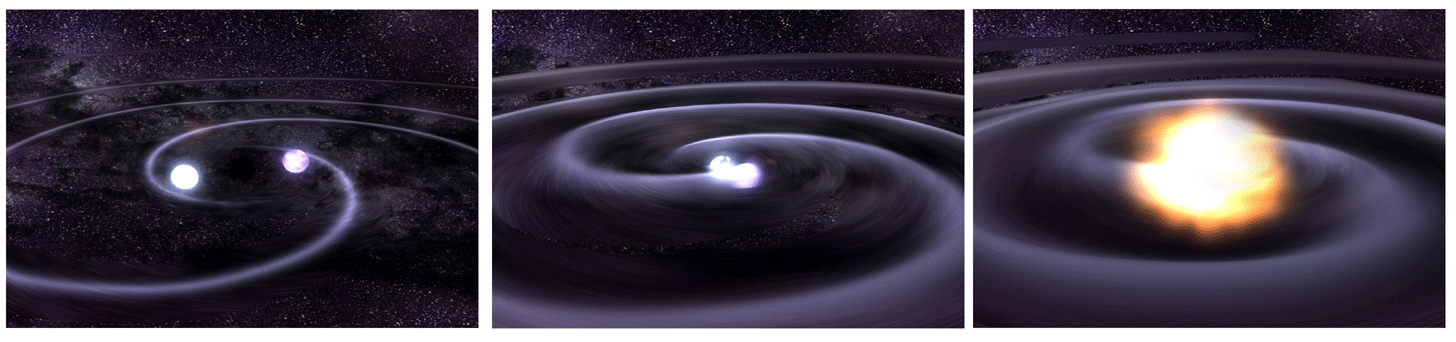
\includegraphics[width=\textwidth]{inspiral_image.jpg}
\end{frame}

\begin{frame}{Detectors}
    \centering
    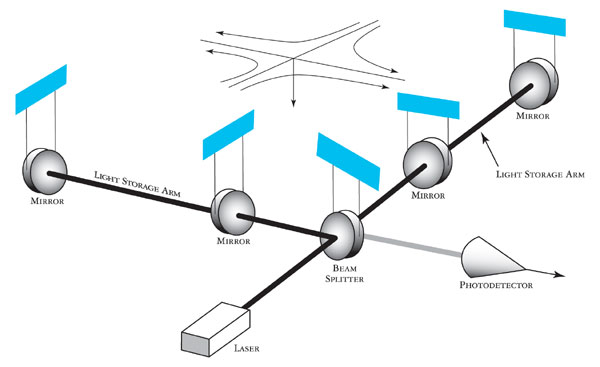
\includegraphics[width=\textwidth]{IFO.jpg}
\end{frame}

\begin{frame}{Processing Pipelines}
    \centering
    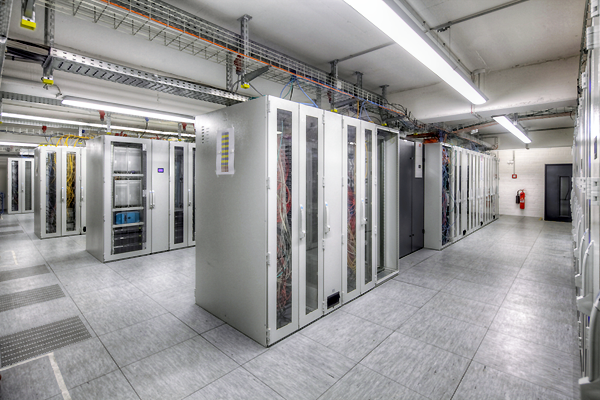
\includegraphics[width=\textwidth]{faq-atlas-cluster.png}
\end{frame}

\begin{frame}{The SPIIR Pipeline}
    \centering
    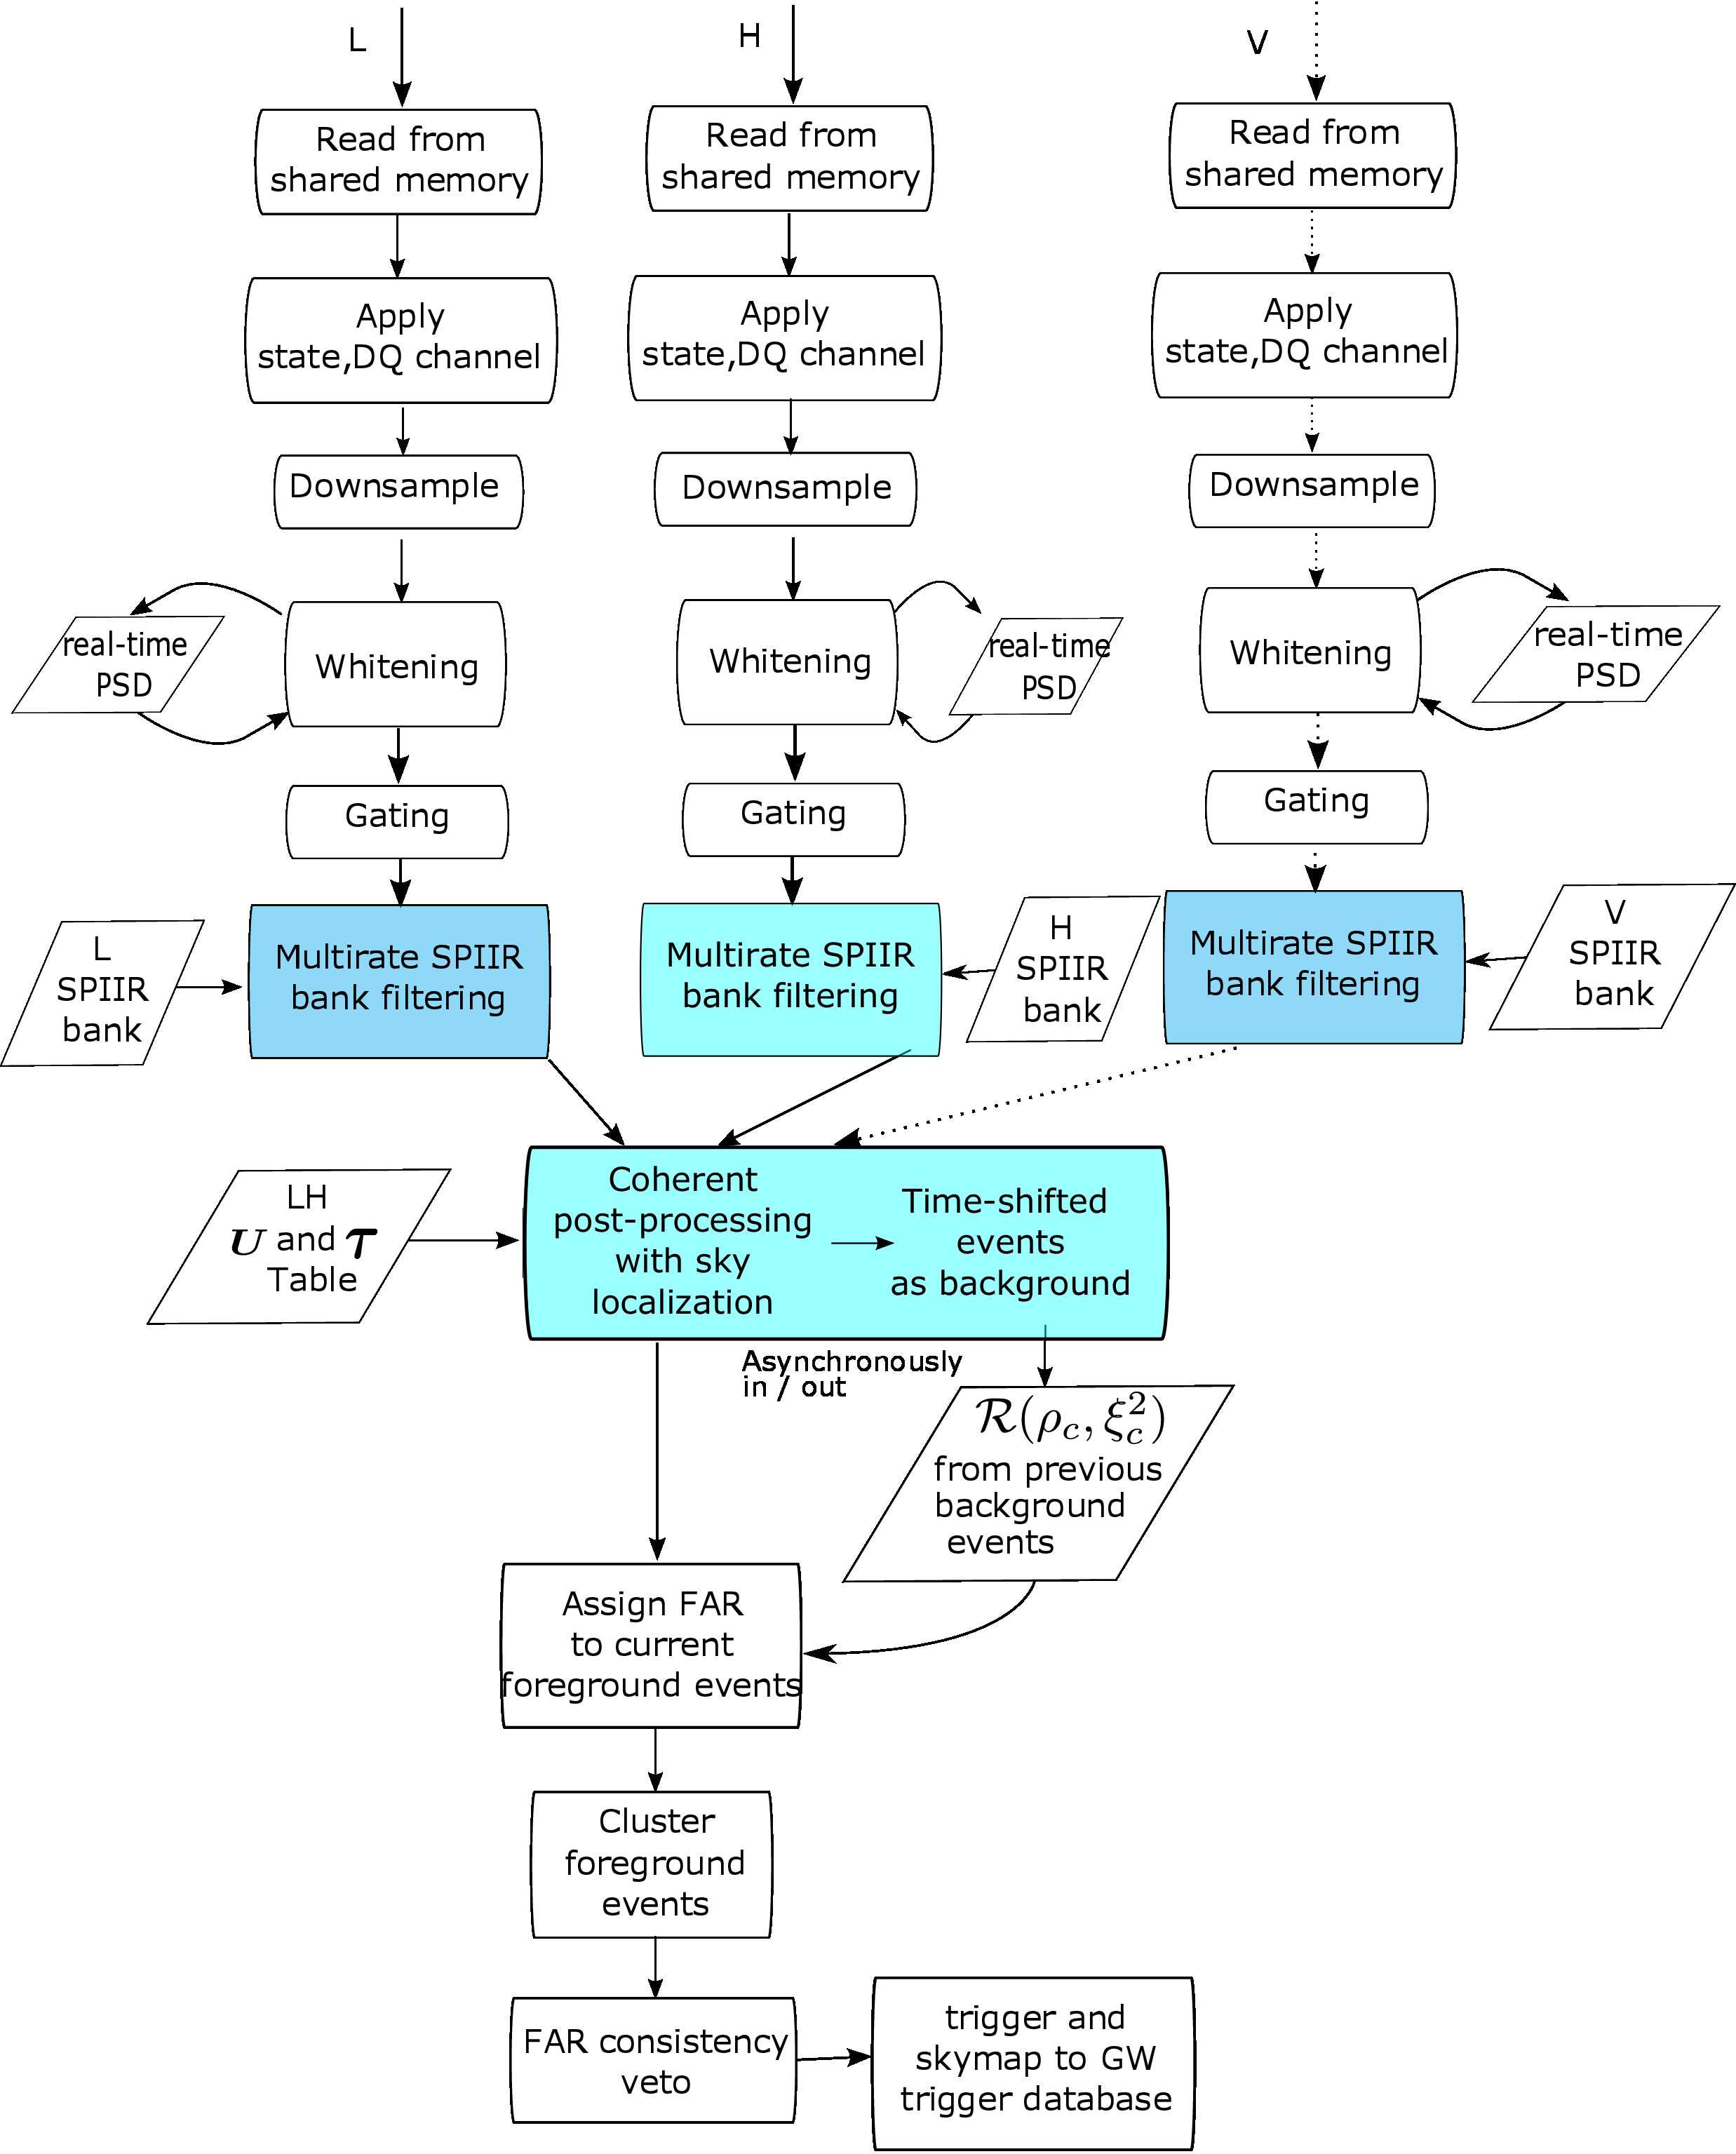
\includegraphics[height=0.7\textheight]{online_xdet.jpg}
\end{frame}

\begin{frame}{The SPIIR Pipeline}
    \centering
    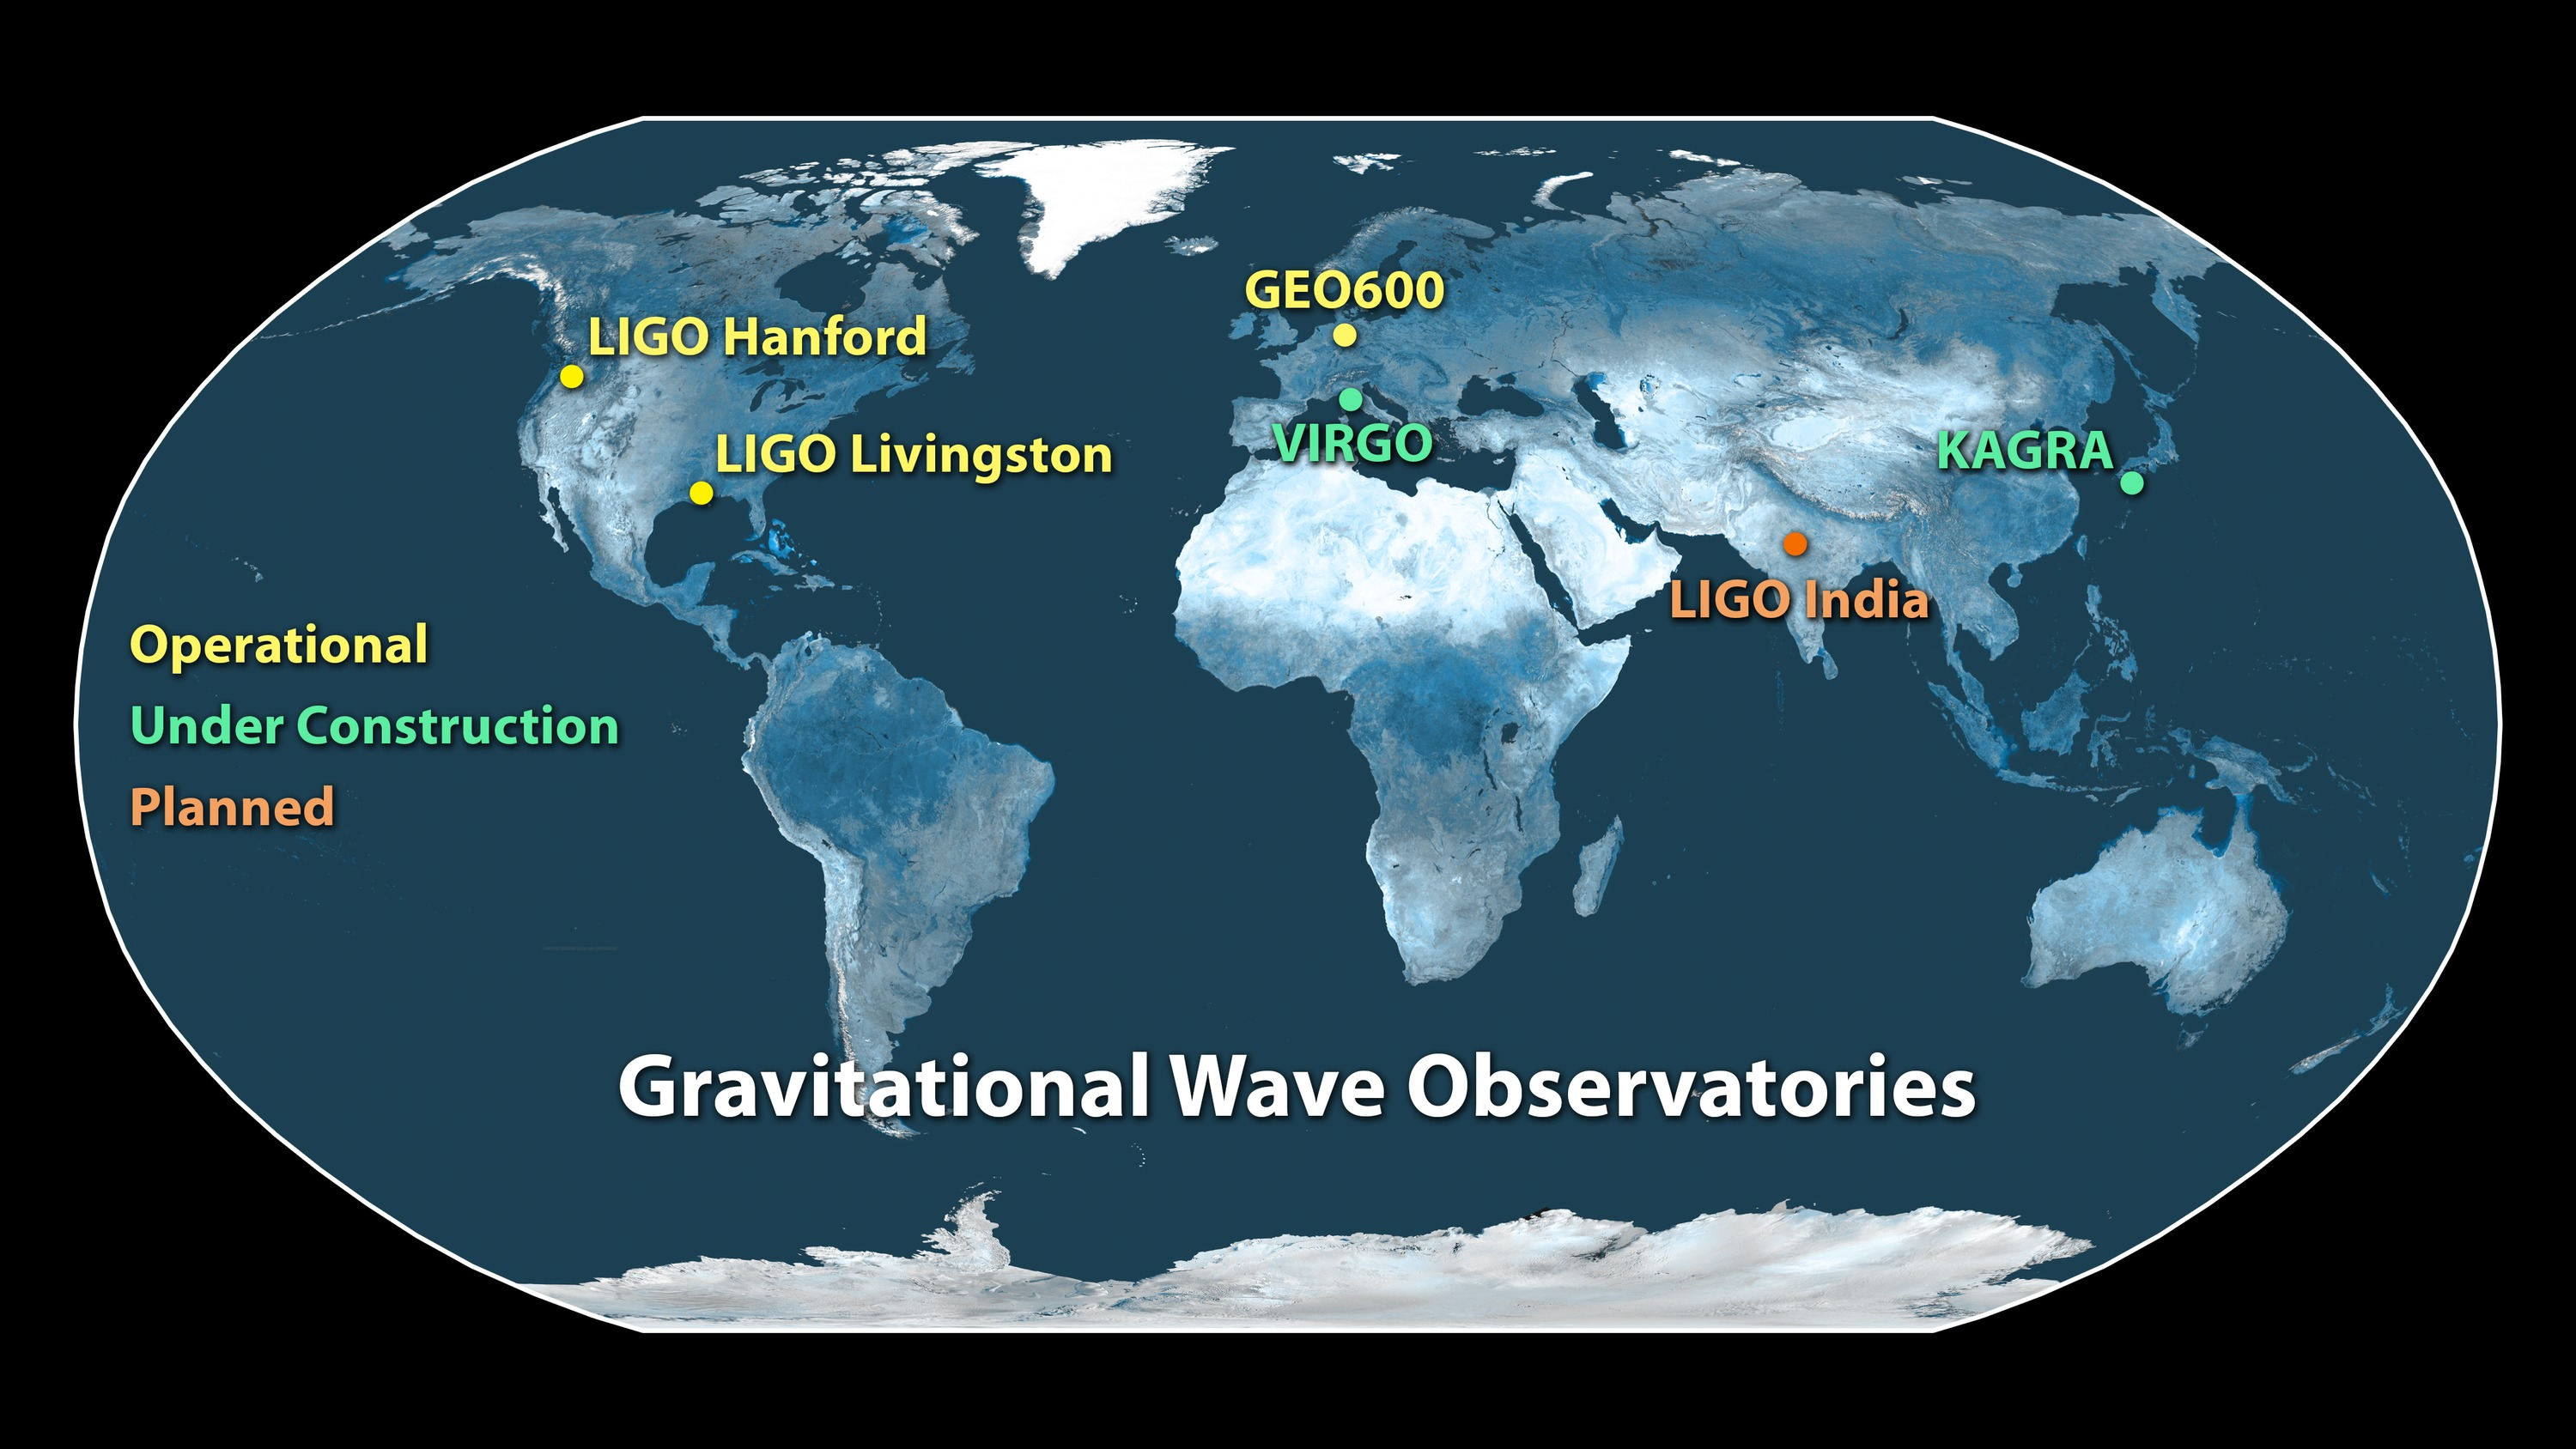
\includegraphics[width=\textwidth]{ligoNetwork-lg.jpg}
\end{frame}

\subsection{The power of powers of 2}

\begin{frame}{Internal datastructures}
    \centering
    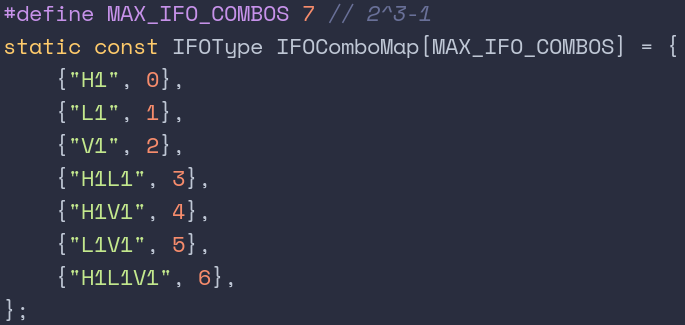
\includegraphics[width=\textwidth]{old-icombo.png}
\end{frame}

\begin{frame}{Internal datastructures}
    \centering
    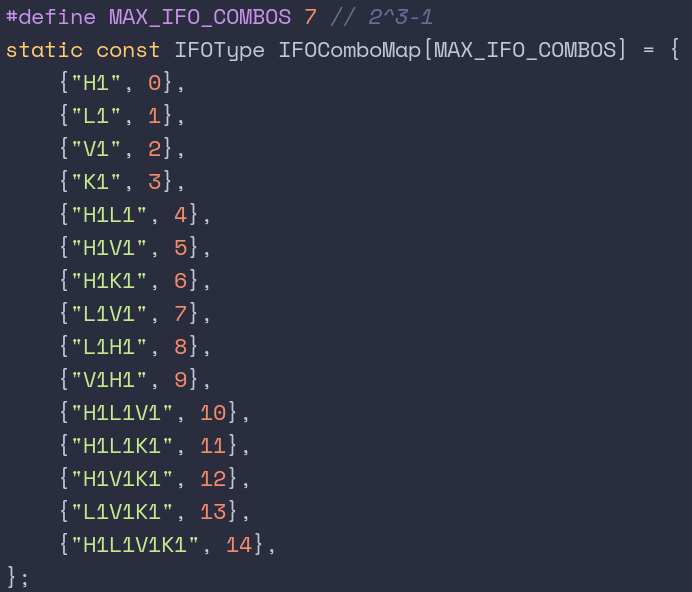
\includegraphics[height=0.75\textheight]{old-icombo-add.png}
\end{frame}

\begin{frame}{Internal datastructures}
    \centering
    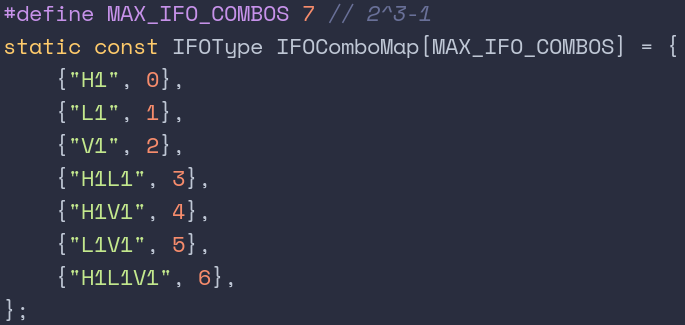
\includegraphics[width=\textwidth]{old-icombo.png}
\end{frame}

\begin{frame}{The power of powers of 2}
    \centering
    \huge{0 0 0 0 0}
\end{frame}

\begin{frame}{The power of powers of 2}
    \centering
    \huge{0 0 0 0 1}
\end{frame}

\begin{frame}{The power of powers of 2}
    \centering
    \huge{0 0 1 0 1}
\end{frame}

\begin{frame}{The power of powers of 2}
    \centering
    \huge{1 0 1 0 1}
\end{frame}

\begin{frame}{The power of powers of 2}
    \centering
    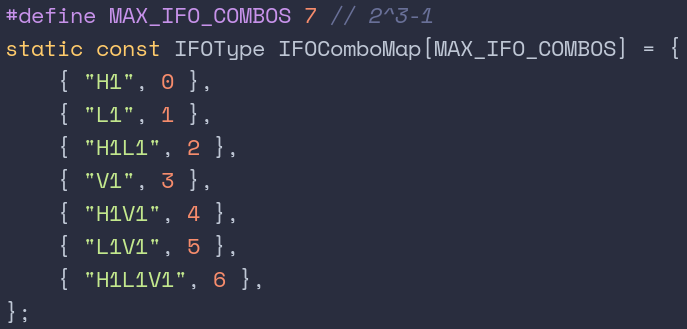
\includegraphics[width=\textwidth]{new-icombo.png}
\end{frame}

\begin{frame}{The power of powers of 2}
    \centering
    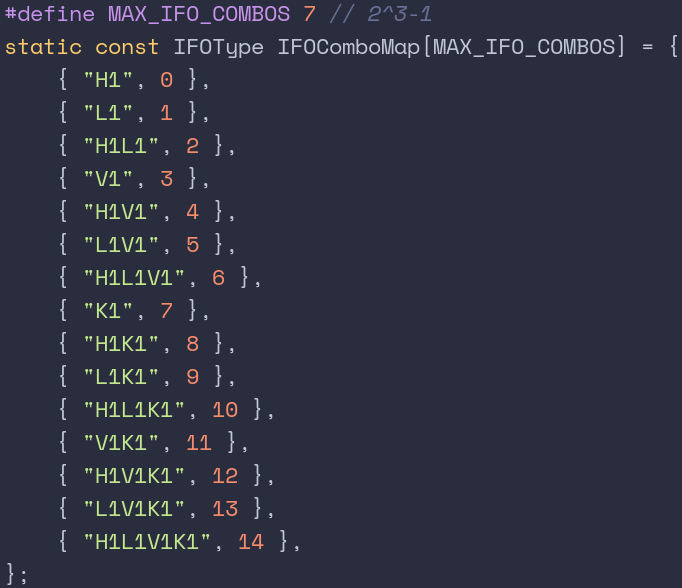
\includegraphics[height=0.75\textheight]{new-icombo-add.png}
\end{frame}

\begin{frame}{The power of powers of 2}
    \centering
    \large{\(N_{detectors} = \) \texttt{popcount(icombo)}}\\
    \large{Detector being used: \texttt{icombo \& \(2^{ifo}\)}}
\end{frame}

\begin{frame}{The power of powers of 2}
    \centering
    
\includegraphics[width=\textwidth]{new-icombo-lines.png}
\end{frame}

\subsection{The hunt for hardcoded detectors}

\begin{frame}{The hunt for hardcoded detectors}
    \centering
    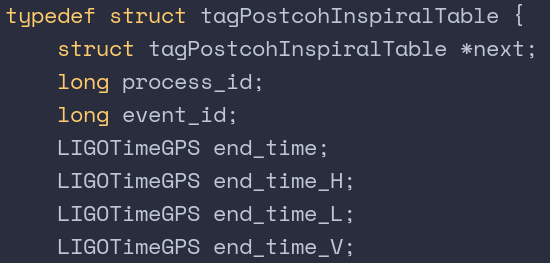
\includegraphics[width=\textwidth]{names-old.png}
\end{frame}

\begin{frame}{The hunt for hardcoded detectors}
    \centering
    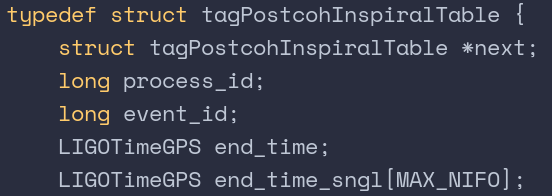
\includegraphics[width=\textwidth]{names-new.png}
\end{frame}

\begin{frame}{The hunt for hardcoded detectors}
    \centering
    
\includegraphics[width=\textwidth]{names-new-lines.png}
\end{frame}

\section{Complexity analysis}

\begin{frame}
  \vfill
  \centering
  \begin{beamercolorbox}[sep=8pt,center,shadow=true,rounded=true]{title}
    \usebeamerfont{title}\insertsectionhead\par%
  \end{beamercolorbox}
  \vfill
\end{frame}


\subsection{Background}

\begin{frame}{Complexity Analysis}
    \centering
    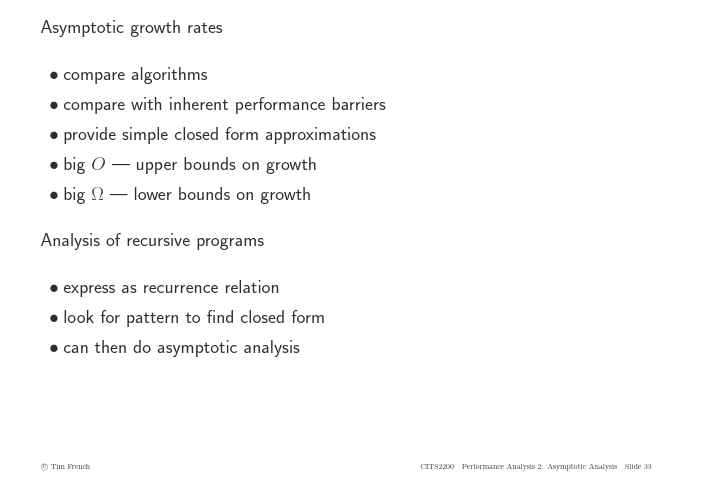
\includegraphics[width=\textwidth]{complexity-definition.png}
\end{frame}

\begin{frame}{Complexity Analysis}
    \centering
    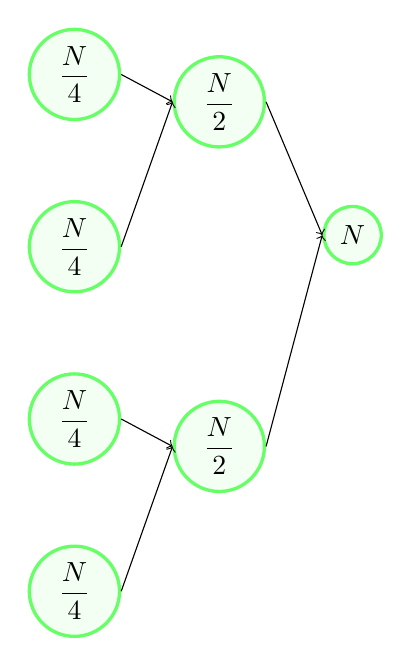
\begin{tikzpicture}[
        selectednode/.style={circle, text=black, draw=red!60, fill=red!5, very thick, minimum size=7mm},
        unselectednode/.style={circle, text=black, draw=green!60, fill=green!5, very thick, minimum size=7mm},
]
        \node[unselectednode] (leftuu) {\(\dfrac{N}{4}\)};
        \node[unselectednode] (leftul) [below=of leftuu] {\(\dfrac{N}{4}\)};
        \node[unselectednode] (leftlu) [below=of leftul] {\(\dfrac{N}{4}\)};
        \node[unselectednode] (leftll) [below=of leftlu] {\(\dfrac{N}{4}\)};
        \node[unselectednode] (centeru) [below right=of leftuu, above right=of leftul] {\(\dfrac{N}{2}\)};
        \node[unselectednode] (centerl) [below right=of leftlu, above right=of leftll] {\(\dfrac{N}{2}\)};
        \node[unselectednode] (right) [above right=of centerl, below right=of centeru] {\(N\)};

        \draw[->] (leftuu.east) -- (centeru.west);
        \draw[->] (leftul.east) -- (centeru.west);
        \draw[->] (leftlu.east) -- (centerl.west);
        \draw[->] (leftll.east) -- (centerl.west);
        \draw[->] (centeru.east) -- (right.west);
        \draw[->] (centerl.east) -- (right.west);
    \end{tikzpicture}
\end{frame}

\begin{frame}{Work}
    \centering
    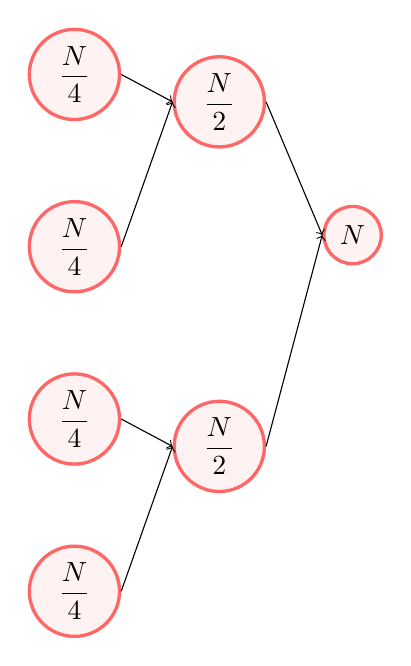
\begin{tikzpicture}[
        selectednode/.style={circle, text=black, draw=red!60, fill=red!5, very thick, minimum size=7mm},
        unselectednode/.style={circle, text=black, draw=green!60, fill=green!5, very thick, minimum size=7mm},
]
        \node[selectednode] (leftuu) {\(\dfrac{N}{4}\)};
        \node[selectednode] (leftul) [below=of leftuu] {\(\dfrac{N}{4}\)};
        \node[selectednode] (leftlu) [below=of leftul] {\(\dfrac{N}{4}\)};
        \node[selectednode] (leftll) [below=of leftlu] {\(\dfrac{N}{4}\)};
        \node[selectednode] (centeru) [below right=of leftuu, above right=of leftul] {\(\dfrac{N}{2}\)};
        \node[selectednode] (centerl) [below right=of leftlu, above right=of leftll] {\(\dfrac{N}{2}\)};
        \node[selectednode] (right) [above right=of centerl, below right=of centeru] {\(N\)};

        \draw[->] (leftuu.east) -- (centeru.west);
        \draw[->] (leftul.east) -- (centeru.west);
        \draw[->] (leftlu.east) -- (centerl.west);
        \draw[->] (leftll.east) -- (centerl.west);
        \draw[->] (centeru.east) -- (right.west);
        \draw[->] (centerl.east) -- (right.west);
    \end{tikzpicture}
\end{frame}

\begin{frame}{Span}
    \centering
    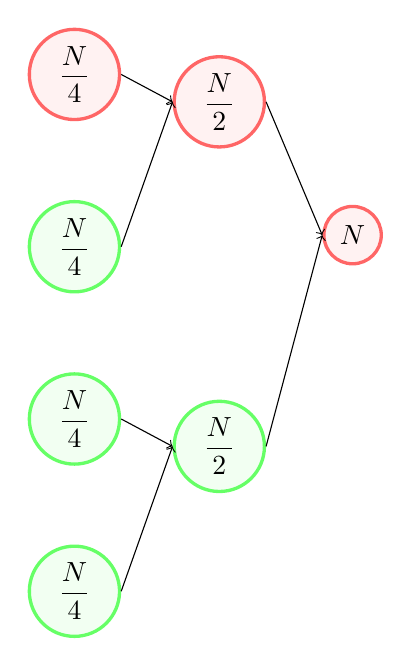
\begin{tikzpicture}[
        selectednode/.style={circle, text=black, draw=red!60, fill=red!5, very thick, minimum size=7mm},
        unselectednode/.style={circle, text=black, draw=green!60, fill=green!5, very thick, minimum size=7mm},
]
        \node[selectednode] (leftuu) {\(\dfrac{N}{4}\)};
        \node[unselectednode] (leftul) [below=of leftuu] {\(\dfrac{N}{4}\)};
        \node[unselectednode] (leftlu) [below=of leftul] {\(\dfrac{N}{4}\)};
        \node[unselectednode] (leftll) [below=of leftlu] {\(\dfrac{N}{4}\)};
        \node[selectednode] (centeru) [below right=of leftuu, above right=of leftul] {\(\dfrac{N}{2}\)};
        \node[unselectednode] (centerl) [below right=of leftlu, above right=of leftll] {\(\dfrac{N}{2}\)};
        \node[selectednode] (right) [above right=of centerl, below right=of centeru] {\(N\)};

        \draw[->] (leftuu.east) -- (centeru.west);
        \draw[->] (leftul.east) -- (centeru.west);
        \draw[->] (leftlu.east) -- (centerl.west);
        \draw[->] (leftll.east) -- (centerl.west);
        \draw[->] (centeru.east) -- (right.west);
        \draw[->] (centerl.east) -- (right.west);
    \end{tikzpicture}
\end{frame}

\begin{frame}{Parallel definitions}
    \begin{itemize}
        \item Work \( = T_1\)
        \item Span \( = T_\infty\)
        \item Brent's Theorem\\
            \(O(\dfrac{T_1}{P} + T_N)\)
    \end{itemize}
\end{frame}

\subsection{So why do we care about this complexity analysis?}

\begin{frame}
  \vfill
  \centering
  \begin{beamercolorbox}[sep=8pt,center,shadow=true,rounded=true]{title}
    \usebeamerfont{title}\insertsubsectionhead\par%
  \end{beamercolorbox}
  \vfill
\end{frame}

\begin{frame}{Why do we care?}
    \centering
    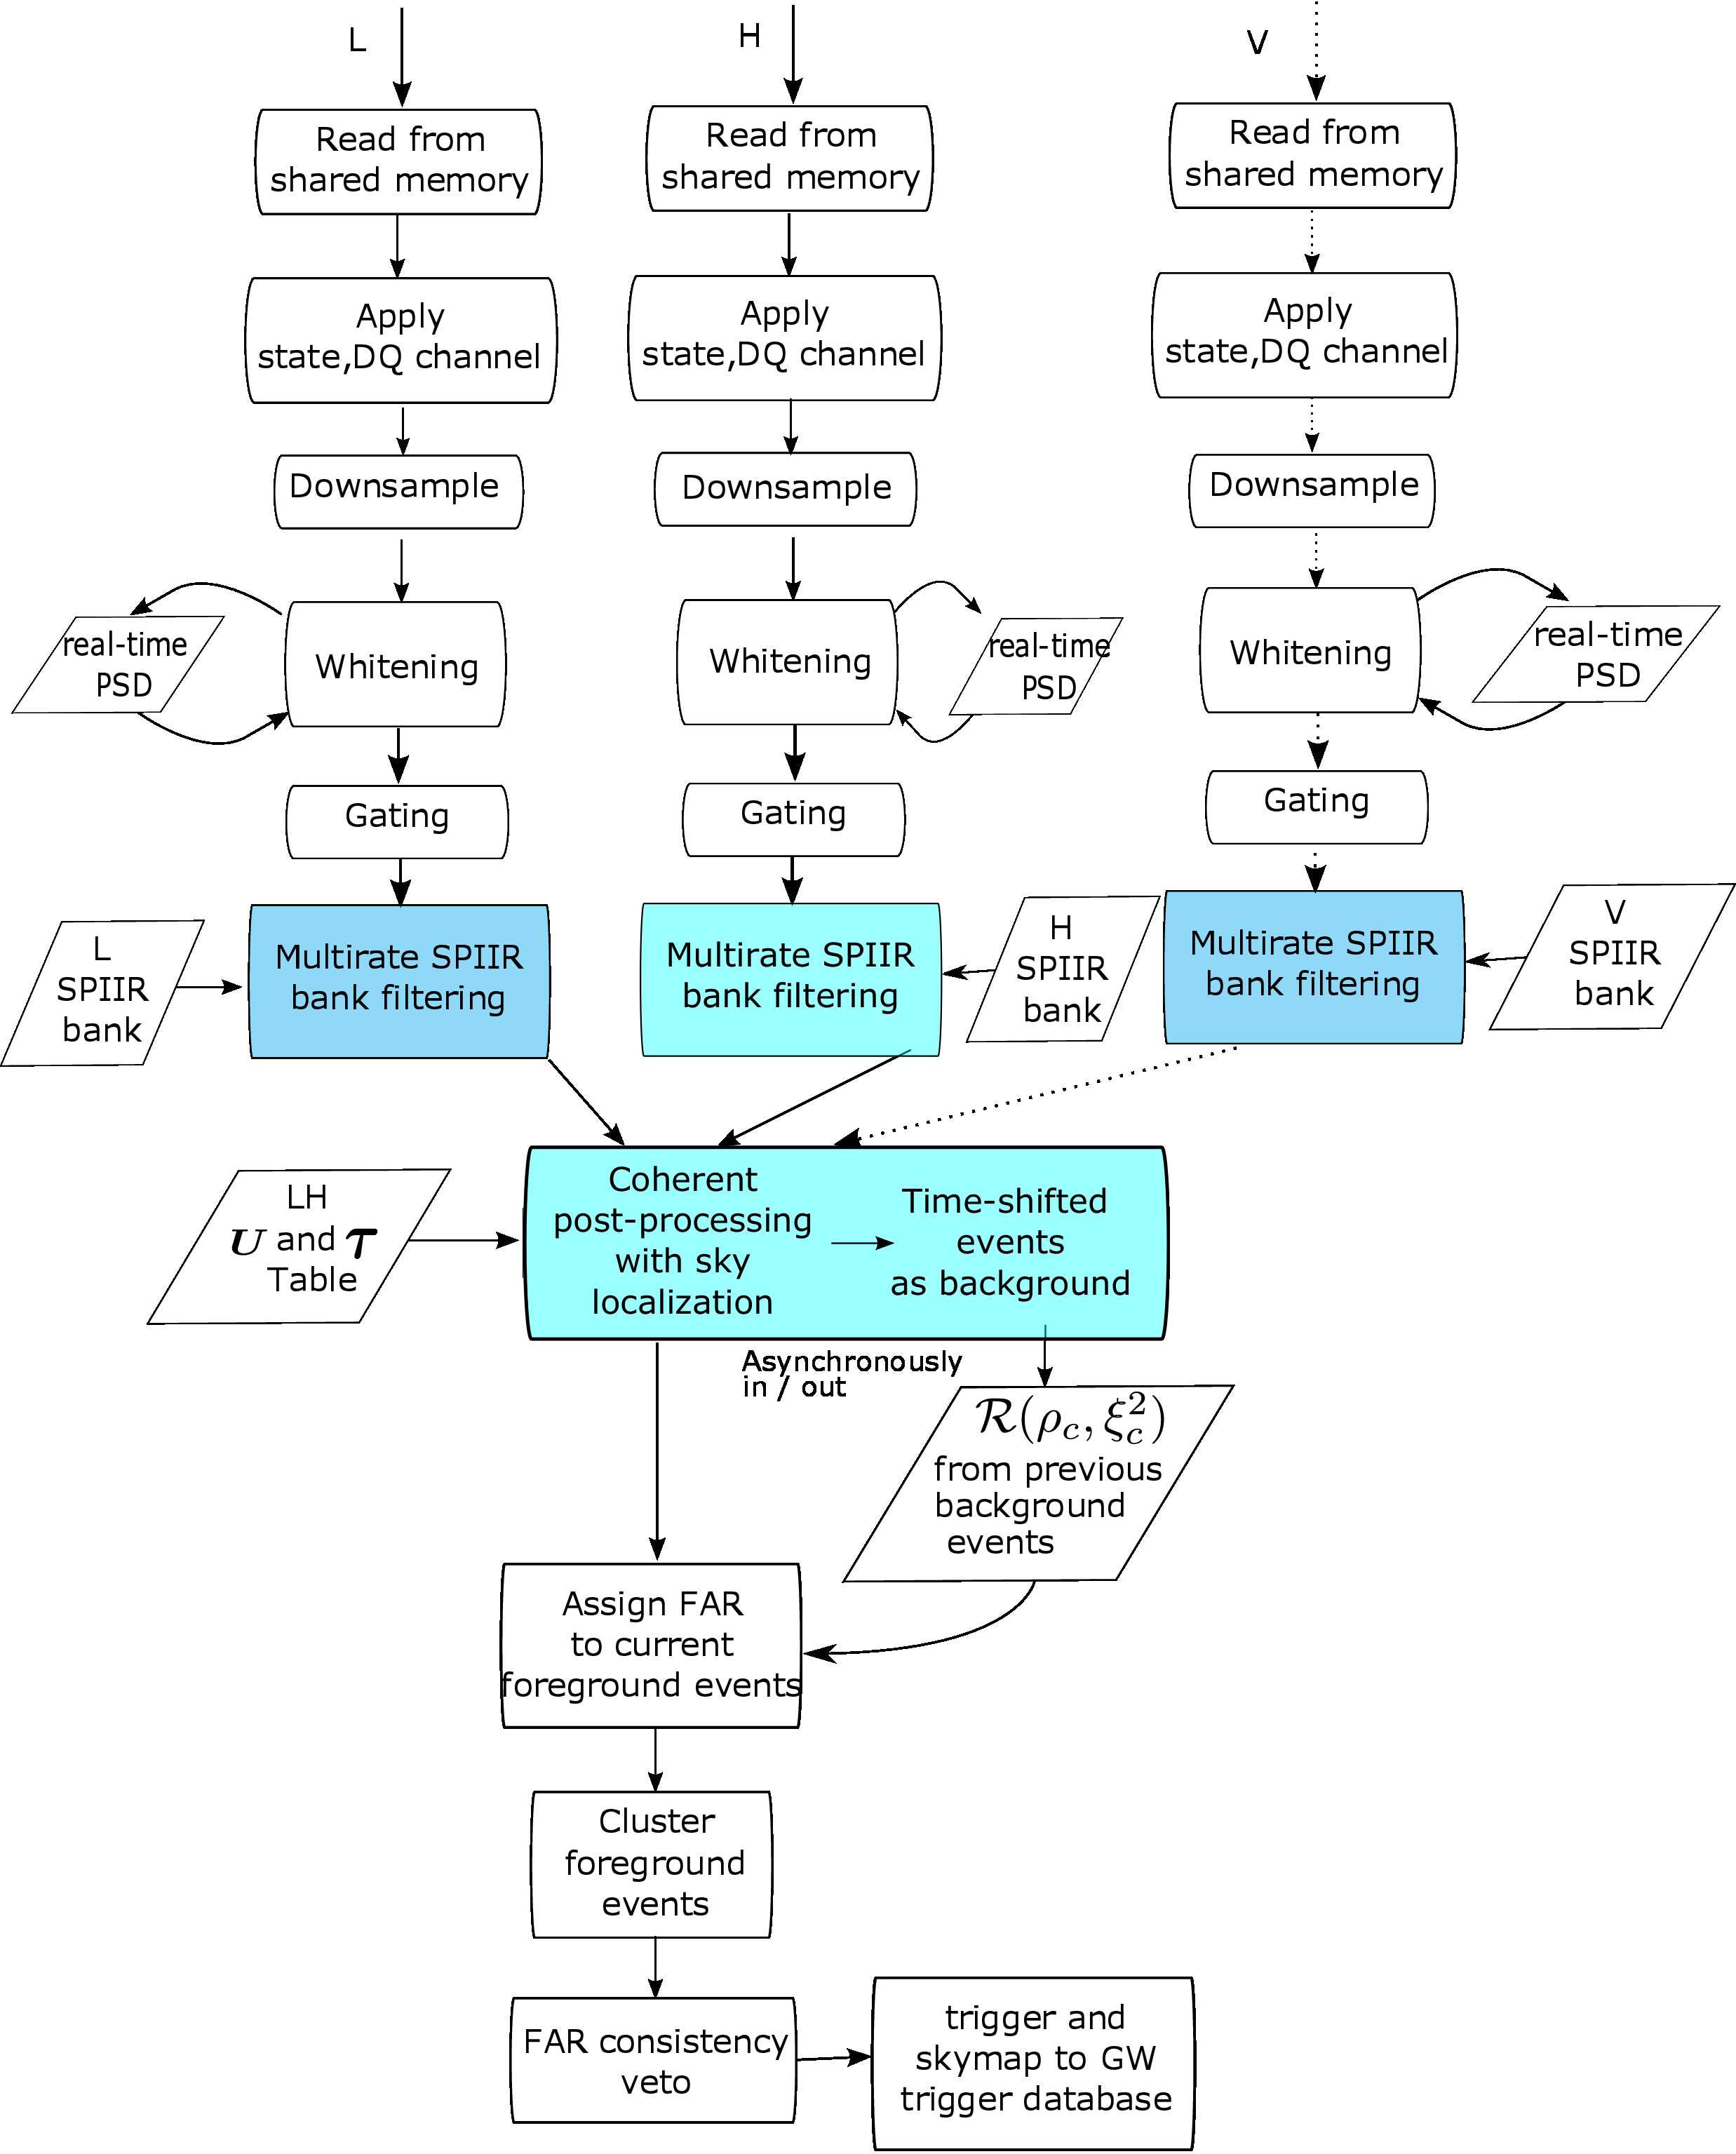
\includegraphics[height=0.7\textheight]{online_xdet.jpg}
\end{frame}

\begin{frame}{Why do we care?}
    \centering
    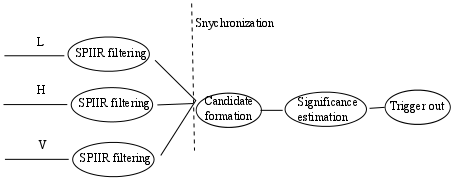
\includegraphics[width=\textwidth]{../resources/current_pipeline.png}
\end{frame}

\subsection{CUDA}

\begin{frame}{CUDA}
    \centering
    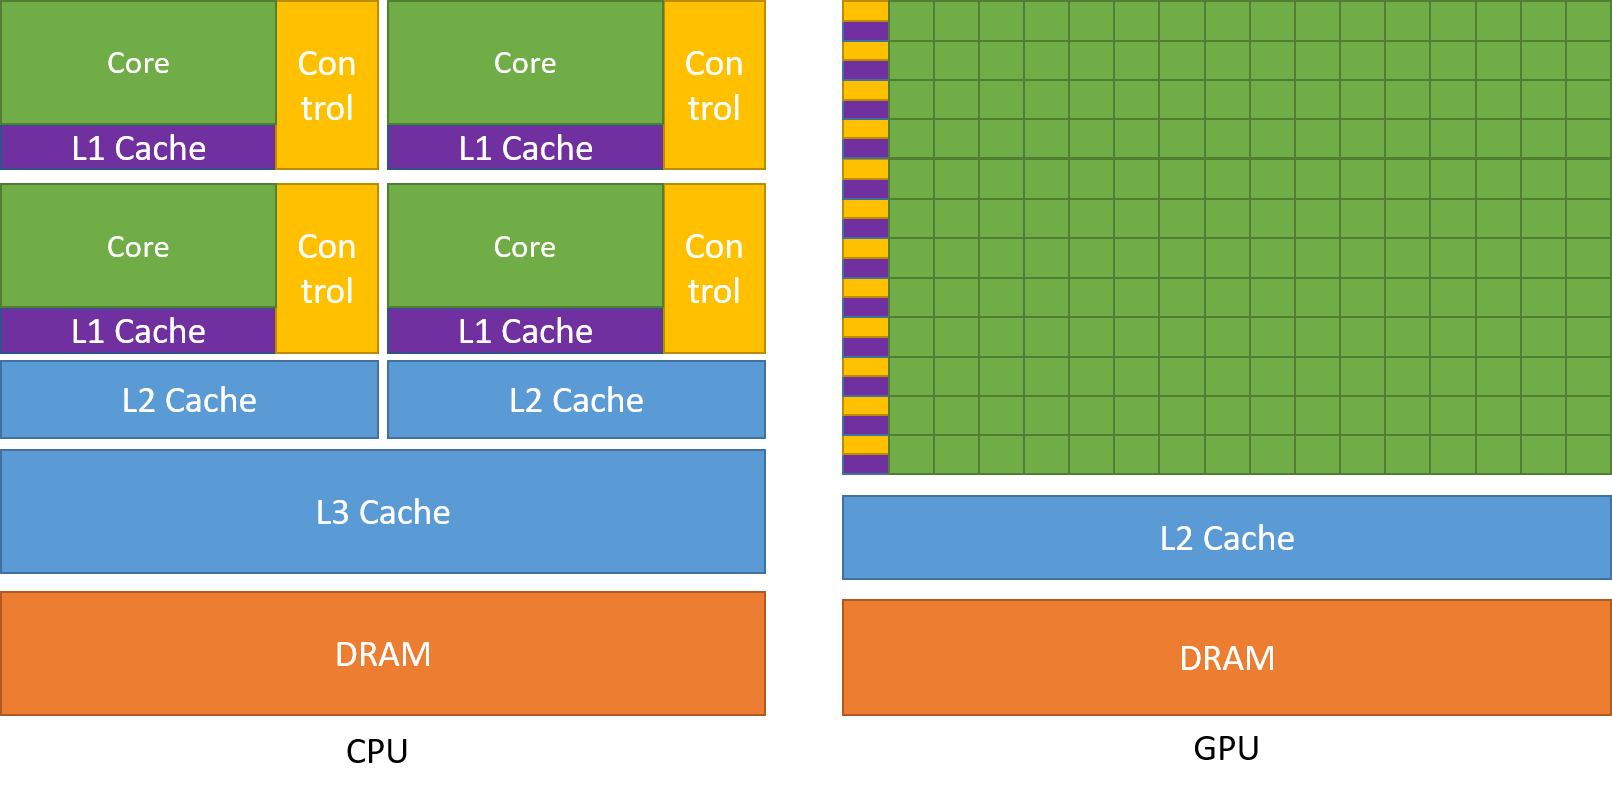
\includegraphics[width=\textwidth]{gpu-cpu.png}
\end{frame}

\begin{frame}{Compute model}
    \centering
    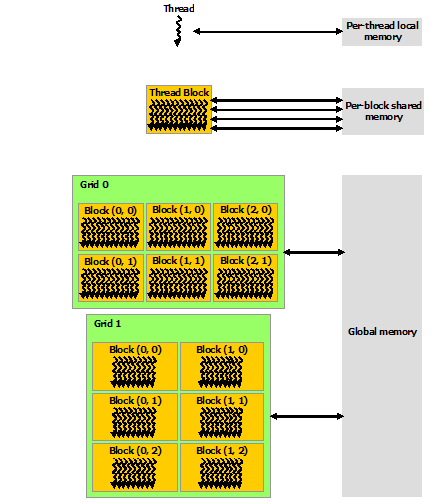
\includegraphics[height=0.7\textheight]{memory-hierarchy.png}
\end{frame}

\subsection{Analysis}

\begin{frame}{Callgraph generation}
    \centering
    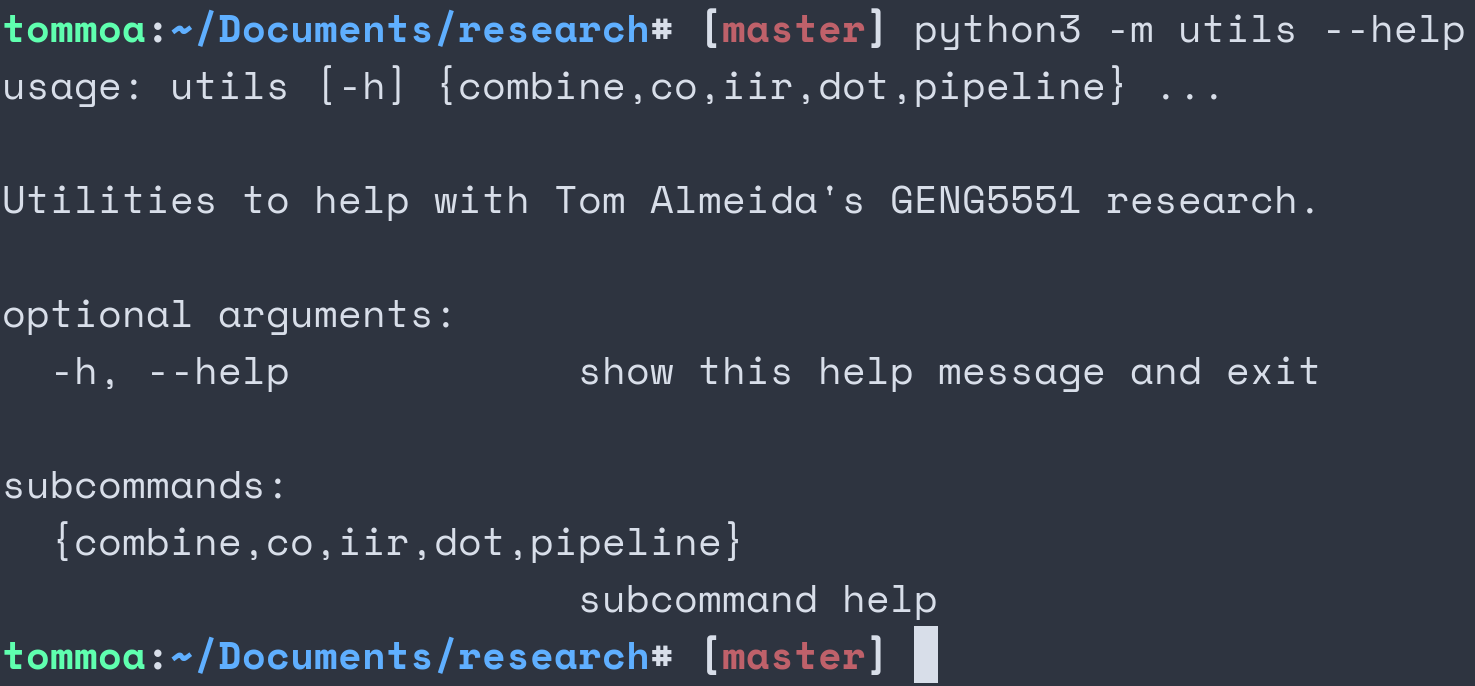
\includegraphics[width=\textwidth]{../progress-report/utils.png}
\end{frame}

\begin{frame}{Callgraph}
    \centering
    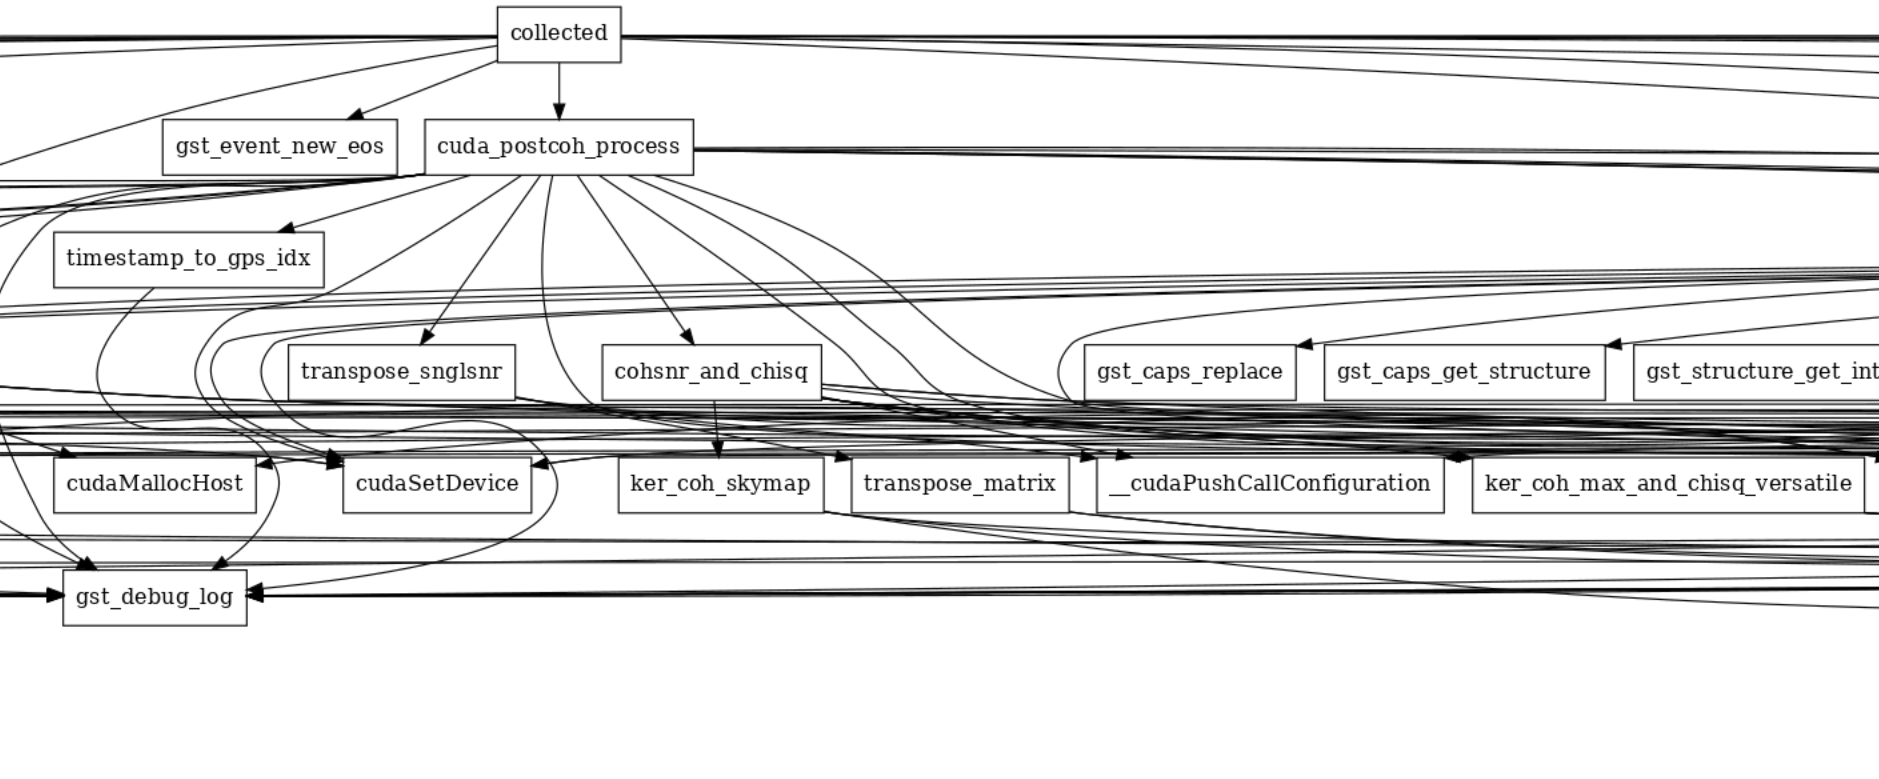
\includegraphics[width=\textwidth]{../progress-report/callgraph.png}
\end{frame}

\begin{frame}{Analysis}
    \begin{itemize}
        \item[\(T_\infty\)] \(= O(NT + N^2 + D^3 + D^2 \log N + D \log S + D \log P)\),
        \item[\(T_1\)] \(= O(NT + N^2 + SPD^3 + SPBD^3 + ND^2)\),
    \end{itemize}
    where \(D\) is the number of detectors,\\
    \(S\) is the number of sky directions,\\
    \(T\) is the number of templates,\\
    \(N\) is the number of samples,\\
    \(B\) is the number of time shifts made to background noise;\\
    and \(P = \max\{S, T\}\).\\
    \centering
    \pause{} \(\dfrac{4^3}{3^3} = \dfrac{64}{27} \approx{} 2.37\)
\end{frame}

\section{Future Work}

\begin{frame}
  \vfill
  \centering
  \begin{beamercolorbox}[sep=8pt,center,shadow=true,rounded=true]{title}
    \usebeamerfont{title}\insertsectionhead\par%
  \end{beamercolorbox}
  \vfill
\end{frame}

\begin{frame}{Pipeline Structure}
    \centering
    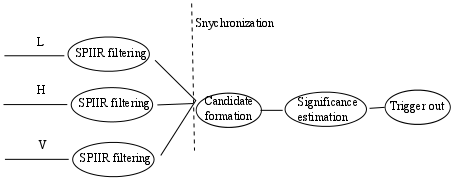
\includegraphics[width=\textwidth]{../resources/current_pipeline.png}
\end{frame}

\begin{frame}{Pipeline Structure}
    \centering
    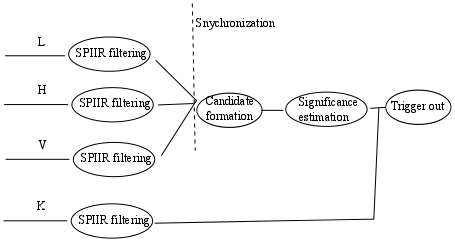
\includegraphics[width=\textwidth]{../resources/new_pipeline.png}
\end{frame}

\begin{frame}{Algorithms}
    \begin{itemize}
        \item[\(T_\infty\)] \(= O(NT + N^2 + D^3 + D^2 \log N + D \log S + D \log P)\),
        \item[\(T_1\)] \(= O(NT + N^2 + SPD^3 + SPBD^3 + ND^2)\),
    \end{itemize}
    where \(D\) is the number of detectors,\\
    \(S\) is the number of sky directions,\\
    \(T\) is the number of templates,\\
    \(N\) is the number of samples,\\
    \(B\) is the number of time shifts made to background noise;\\
    and \(P = \max\{S, T\}\).\\
    \centering
    \pause{} \(\dfrac{4^2}{3^2} = \dfrac{16}{9} \approx{} 1.78\)
\end{frame}

\begin{frame}
  \vfill
  \centering
  \begin{beamercolorbox}[sep=8pt,center,shadow=true,rounded=true]{title}
    \usebeamerfont{title}Questions?\par%
  \end{beamercolorbox}
  \vfill
\end{frame}

\end{document}
